\documentclass[a4paper,12pt,oneside]{article}

\usepackage[left=1.0in, right=1.0in, top=1.0in, bottom=1.0in]{geometry}

\usepackage[toc,page]{appendix}
\usepackage{amsmath}
\usepackage{amsfonts}
\usepackage{amssymb}
\usepackage{amsthm}
\usepackage{color}
\usepackage{graphics}
\usepackage{graphicx}
\usepackage{epsfig}
\usepackage{epstopdf}
\epstopdfsetup{update}
\usepackage{float}
\usepackage{rotating}
\usepackage{array}
\usepackage{textcomp}
\usepackage{bbm}
\usepackage{fancyref}
\usepackage{xcolor}
\usepackage{rotating}
\usepackage[noadjust]{cite} % basic fos bibliography [1]-[5]
\usepackage{bm}
\usepackage{mathtools}
\usepackage{multirow}
\usepackage{array}
\usepackage{longtable}
\usepackage{hhline}
\usepackage{indentfirst}
\usepackage{framed}
\usepackage[hidelinks]{hyperref}
\usepackage{tcolorbox}
\usepackage{tikz}
\usetikzlibrary{calc,positioning,shapes,shadows,arrows,fit}

\usepackage{environ}
\NewEnviron{graybox}{%
  \begin{tcolorbox}[colback=black!30, colframe=white!80!]
    \BODY
  \end{tcolorbox}
}



%\usepackage{fontspec}
%\setmainfont{cmr12}


%\usepackage{algorithm}
%\usepackage{algpseudocode}
%\usepackage{algcompatible}
%\usepackage{pifont}
%\usepackage[]{algorithm2e}
%\usepackage{stmaryrd}
%\usepackage{subcaption}


\theoremstyle{definition}
\newtheorem{definition}{Definition}[section] %definition
\newtheorem{remark}{Remark}[section] % remark
\newtheorem{theorem}{Theorem}[section] % theorem
\newtheorem{example}{Example}[section] % example
\newtheorem{assumption}{Assumption}[section] % example
\newtheorem{problem}{Problem}[section]

%\newtheorem{theorem}{Theorem}[section] % theorem


\newcolumntype{C}[1]{>{\centering\let\newline\\\arraybackslash}m{#1}}

\makeatletter
\def\BState{\State\hskip-\ALG@thistlm}
\makeatother

\newcommand*{\mybox}[2]
{
  \noindent\colorbox{#1!30}{
  \parbox{0.98\linewidth}{#2}}
}

\newcommand{\note}[1]{{\color{red}  #1}}
\newcommand{\mat}[1]{\bm{\mathit{#1}}}
\newcommand{\vect}[1]{\bm{\mathbf{#1}}}




%\hypersetup{colorlinks=false, linkbordercolor={0 0 1}}












\title{\textbf{Multi-Robot Control by
Utilizing Distributed Model Predictive Controllers}}
%
\author{KTH Royal Institute of Technology \\
  School of Electrical Engineering \\
  Department of Automatic Control \\ \\
Student: Alexandros Filotheou (\href{mailto: alefil@kth.se}{alefil@kth.se}) \\
Supervisor: Alexandros Nikou (\href{mailto: anikou@kth.se}{anikou@kth.se}) \\
Examiner: Dimos Dimarogonas (\href{mailto: dimos@kth.se}{dimos@kth.se}) \\}

\date{\today}

\begin{document}

\maketitle

\begin{abstract}
	This paper addresses the problem of position- and orientation-based formation
  control of a class of second-order nonlinear multi-agent systems in $3$D
  space, under static and undirected communication topologies. More
  specifically, we design a decentralized control protocol for each agent in
  the sense that each agent uses only local information from its neighbors to
  calculate its own control signal. Additionally, by introducing certain
  inter-agent distance constraints, we guarantee collision avoidance both
  between among the agents and between the agents and possible obstacles of the
  workspace. Connectivity maintenance between agents that are initially
  connected is also achieved by the proposed controller scheme. Finally,
  simulation results verify the  performance of the proposed controllers.
\end{abstract}

\newpage
\tableofcontents
\newpage


\section{Introduction}

  \noindent formation of multi-agent systems, mpc intro etc. \\

\noindent motivation why we need mpc controllers...  \\

\noindent In many control problems it is desired to design a stabilizing
feedback such that a performance criterion is minimized while satisfying
constraints on the controls and the states. Ideally one would look for a
closed solution for the feedback law satisfying the constraints while
optimizing the performance. However, typically the optimal feedback law
cannot be found analytically, even in the unconstrained case, since it involves
the solution of the corresponding Hamilton-Jacobi-Bellman partial differential
equations. One approach to circumvent this problem is the repeated solution of
an open-loop optimal control problem for a given state. The first part of the
resulting open-loop input signal is implemented and the whole process is
repeated. Control approaches using this strategy are referred to as Model
Predictive Control (MPC).

  \newpage


\section{Notation and Preliminaries} \label{sec:notation_reliminaries}

  \subsection{Notation}

The set of positive integers is denoted as $\mathbb{N}$. The real $n$-coordinate
space, with $n\in\mathbb{N}$, is denoted as $\mathbb{R}^n$;
$\mathbb{R}^n_{\geq 0}$ and $\mathbb{R}^n_{> 0}$ are the sets of real
$n$-vectors with all elements nonnegative and positive, respectively. Given a
set $S$, we denote as $\lvert S\lvert$ its cardinality. The notation $\|x\|$
is used for the Euclidean norm of a vector $x \in \mathbb{R}^n$. Given a
symmetric matrix $A, \lambda_{\text{min}}(A) = \min \{|\lambda| : \lambda \in \sigma(A) \}$
denotes the minimum eigenvalue of $A$, respectively, where $\sigma(A)$ is the
set of all the eigenvalues of $A$ and $\text{rank}(A)$ is its rank;
$A \otimes B$ denotes the Kronecker product of matrices $A, B \in \mathbb{R}^{m \times n}$,
as was introduced in \cite{horn_jonshon}. Define by $\mathbbm{1}_n \in \mathbb{R}^n, I_n \in \mathbb{R}^{n \times n}, 0_{m \times n} \in \mathbb{R}^{m \times n}$
the column vector with all entries $1$, the unit matrix and the $m \times n$
matrix with all entries zeros, respectively.
A matrix $A \in \mathbb{R}^{n \times n}$ is called skew-symmetric if and only
if $A^\top = -A$. $\mathcal{B}(c,r) = \{x \in \mathbb{R}^3: \|x-c\| \leq r\}$
is the $3$D sphere of radius $r \in \mathbb{R}_{\ge 0}$ and center
$c\in\mathbb{R}^{3}$.
The vector connecting the origins of coordinate frames $\{A\}$ and $\{B$\}
expressed in frame $\{C\}$ coordinates in $3$D space is denoted as
$p^{\scriptscriptstyle C}_{{\scriptscriptstyle B/A}}\in{\mathbb{R}}^{3}$.
Given $a\in\mathbb{R}^3$, $S(a)$ is the skew-symmetric matrix
defined according to $S(a)b = a\times b$. We further denote as
$q_{\scriptscriptstyle B/A}\in\mathbb{T}^3$ the Euler angles representing
the orientation of frame $\{B\}$ with respect to frame $\{A\}$, where
$\mathbb{T}^3$ is the $3$D torus. The angular velocity of frame $\{B\}$ with
respect to $\{A\}$, expressed in frame $\{C\}$ coordinates, is denoted as
$\omega^{\scriptscriptstyle C}_{\scriptscriptstyle B/A}\in \mathbb{R}^{3}$.
We also use the notation $\mathbb{M} = \mathbb{R}^3\times \mathbb{T}^3$.
For notational brevity, when a coordinate frame corresponds to an inertial frame
of reference $\{0\}$, we will omit its explicit notation
(e.g., $p_{\scriptscriptstyle B} = p^{\scriptscriptstyle 0}_{\scriptscriptstyle B/0},
\omega_{\scriptscriptstyle B} = \omega^{\scriptscriptstyle 0}_{\scriptscriptstyle B/0}$ etc.).
All vector and matrix differentiations are derived with respect to an inertial
frame $\{0\}$, unless otherwise stated.

\subsection{Graph Theory}

An \textit{undirected graph} $\mathcal{G}$ is a pair
$(\mathcal{V}, \mathcal{E})$, where $\mathcal{V}$ is a finite set of nodes,
representing a team of agents, and
$\mathcal{E} \subseteq \{ \{i,j\} : i,j \in \mathcal{V}, i \neq j\}$,
with $M = |\mathcal{E}|$, is the set of edges that model the communication
capability between neighboring agents. For each agent, its neighbors' set
$\mathcal{N}_i$ is defined as
$\mathcal{N}_i = \{i_1, \ldots, i_{N_i}\} = \{ j \in \mathcal{V} : \{i,j\} \in \mathcal{E}\}$,
where $i_1, \ldots, i_{N_i}$ is an enumeration of the neighbors of agent $i$
and $N_i = |\mathcal N_i|$.

If there is an edge $\{i, j\} \in \mathcal{E}$, then $i, j$ are called
\textit{adjacent}. A \textit{path} of length $r$ from vertex $i$ to vertex
$j$ is a sequence of $r+1$ distinct vertices, starting with $i$ and ending
with $j$, such that consecutive vertices are adjacent. For $i = j$, the path
is called a \text{cycle}. If there is a path between any two vertices of the
graph $\mathcal{G}$, then $\mathcal{G}$ is called \textit{connected}.
A connected graph is called a \text{tree} if it contains no cycles.

  \newpage


\section{Problem Formulation} \label{sec:prob_formulation}

  \subsection{System Model}
Consider a set of $N$ rigid bodies, with $\mathcal{V} = \{ 1,2, \ldots, N\}$,
$N  \geq 2$, operating in a workspace $W\subseteq \mathbb{R}^3$, with coordinate
frames $\{i\}, i\in\mathcal{V}$, attached to their centers of mass. The
workspace is assumed to be modeled as a bounded sphere $\mathcal{B}(0,r_w)$.
We consider that each agent occupies a sphere $\mathcal{B}(p_i(t), r_i)$,
where $p_i:\mathbb{R}_{\geq 0} \to \mathbb{R}^3$ is the position of the agent's
center of mass and $r_i$ is the agent's radius. We also denote as
$q_i:\mathbb{R}_{\geq 0} \to \mathbb{T}^3, i\in\mathcal{V}$, the Euler angles
representing the agents' orientation with respect to an inertial frame $\{0\}$,
with $q_i = [\phi_i,\theta_i,\psi_i]^\tau$.
By defining $x_i:\mathbb{R}_{\geq 0} \to \mathbb{M}, v_i : \mathbb{R}_{\geq 0} \to \mathbb{R}^6$,
with $x_i = [p^\tau_i,q^\tau_i]^\tau, v_i =[\dot{p}^\tau_i,\omega^\tau_i]^\tau$,
we model each agent's motion with the $2$nd order dynamics:

\begin{subequations}\label{eq:system}
	\begin{align}
	& \dot{x}_i(t) = J_i(x_i)v_i(t) , \label{eq:system_1} \\
	& M_i(x_i) \dot{v}_i(t) + C_i(x_i,\dot{x}_i) v_i(t)+g_i(x_i) = u_i,  \label{eq:system_2}
	\end{align}
\end{subequations}
where $J_i:\mathbb{M} \to \mathbb{R}^{6\times6}$ is a Jacobian matrix that maps
the Euler angle rates to $v_i$, given by
\begin{align}
J_i(x_i)
&=
\begin{bmatrix}
I_3 & 0_{3 \times 3} \\
0_{3 \times 3} & J_{ q }(x_i) \\
\end{bmatrix} \notag, \\
J_q(x_i)
&=
\begin{bmatrix}
1 & \sin(\phi_i) \tan(\theta_i)  & \cos(\phi_i) \tan(\theta_i) \\
0 & \cos(\phi_i) & -\sin(\phi_i) \\
0  & \displaystyle \frac{\sin(\phi_i)}{\cos(\theta_i)} & \displaystyle \frac{\cos(\phi_i)}{\cos(\theta_i)}
\end{bmatrix}, \notag
\end{align}

for which we make the following assumption:

\begin{assumption} \label{as:J}
	The angle $\theta_i$ satisfies the inequality
  $-\frac{\pi}{2} < \theta_i(t) < \frac{\pi}{2} ,\forall i\in\mathcal{V},t\in\mathbb{R}_{\geq 0}$.
\end{assumption}

The aforementioned assumption guarantees that $J_i$ is always well-defined and
invertible, since $\det(J_i) = \tfrac{1}{\cos\theta_i}$.
Furthermore, $M_i:\mathbb{M} \to \mathbb{R}^{6\times6}$ is the symmetric and
positive definite inertia matrix,
$C_i:\mathbb{M}\times\mathbb{R}^6 \to \mathbb{R}^{6\times6}$ is the Coriolis
matrix and $g_i:\mathbb{M} \to \mathbb{R}^6$ is the gravity vector.
We consider that the aforementioned vector fields are unknown and continuous.
Finally, $u_i\in\mathbb{R}^6$ is the control input vector representing the $6$D
generalized force acting on the agent. Let as also define the vectors
$x = [x_1^\tau,\dots,x_N^\tau]^\tau : \mathbb{R}_{\geq 0} \to \mathbb{M}^N, v = [v_1^\tau, \dots$
and $v_N^\tau]^\tau : \mathbb{R}_{\geq 0} \to \mathbb{R}^{6N}$.

\begin{remark}
	According to \cite{Siciliano2009}, the matrices
  $\dot{M}_i-C_i, i \in \mathcal{V}$ are skew-symmetric.
  From \cite{horn_jonshon}, we have that a quadratic form of a skew-symmetric
  matrix is always equal to $0$. Hence, for the matrices $\dot{M}_i-C_i$ it
  holds that:

	\begin{equation} \label{eq:skew_symm}
	y^\top \left[\dot{M}_i - 2 C_i\right]y = 0, \forall y \in \mathbb{R}^n, i \in \mathcal{V}.
	\end{equation}

\end{remark}

\begin{figure}[ht!]
	\centering
	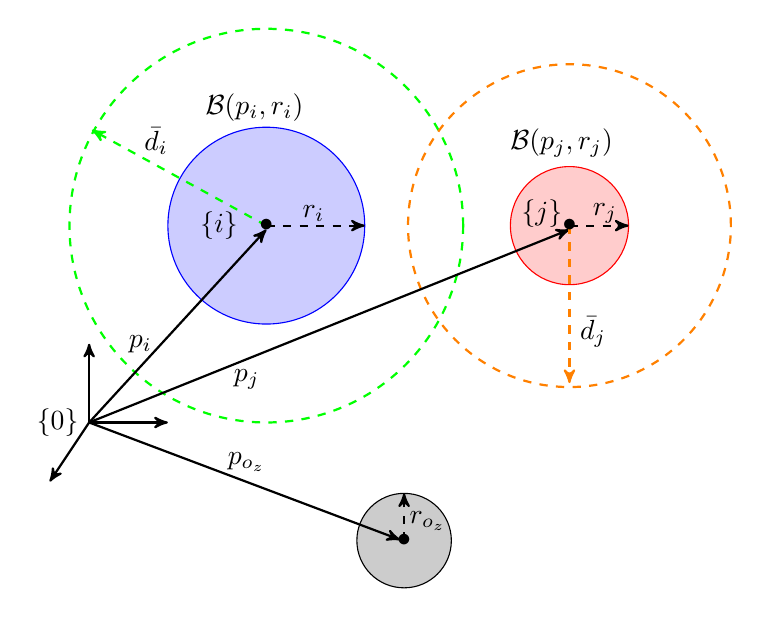
\begin{tikzpicture}[scale = 0.5]
	%draw the global frame
	\draw [color=black,thick,->,>=stealth'](-9, -5) to (-7, -5);
	\draw [color=black,thick,->,>=stealth'](-9, -5) to (-9, -3);
	\draw [color=black,thick,->,>=stealth'](-9, -5) to (-10, -6.5);
	\node at (-9.8, -5.0) {$\{0\}$};

	%draw agent i
	\draw [color = blue, fill = blue!20] (-4.5,0) circle (2.5cm);
	\node at (-5.7, 0.0) {$\{i\}$};
	\draw[green,thick,dashed] (-4.5,0) circle (5.0cm);
	\draw [color=black,thick,->,>=stealth'](-9, -5) to (-4.5, -0.1);
	\node at (-7.7, -3.0) {$p_i$};
	\draw [color=green,thick,dashed,->,>=stealth'](-4.5, 0.0) to (-8.93, 2.43);
	\node at (-7.3, 2.15) {$\bar{d}_i$};
	\draw [color=black,thick,dashed,->,>=stealth'](-4.5, 0.0) to (-2.0, 0.0);
	\node at (-3.3, 0.3) {$r_i$};
	\node at (-4.5, 0.0) {$\bullet$};
	\node at (-4.8, 3.0) {$\mathcal{B}(p_i, r_i)$};

	%draw agent j
	\draw [color = red, fill = red!20] (3.2, 0) circle (1.5cm);
	\node at (2.5, 0.3) {$\{j\}$};
	\draw[orange,thick,dashed,] (3.2, 0) circle (4.1cm);
	\draw [color=black,thick,->,>=stealth'](-9, -5) to (3.2, -0.1);
	\node at (-5.0, -3.9) {$p_j$};
	\draw [color=orange,thick,dashed,->,>=stealth'](3.2, 0.0) to (3.2, -4.0);
	\node at (3.8, -2.7) {$\bar{d}_j$};
	\draw [color=black,thick,dashed,->,>=stealth'](3.2, 0.0) to (4.7, 0.0);
	\node at (4.1, 0.3) {$r_j$};
	\node at (3.2, 0.0) {$\bullet$};
	\node at (3.0, 2.1) {$\mathcal{B}(p_j, r_j)$};

	% draw the obstacle
	\draw [color = black, fill = black!20] (-1, -8) circle (1.2cm);
	\draw [color=black,thick,->,>=stealth'](-9, -5) to (-1.1, -7.98);
	\draw [color=black,thick,dashed,->,>=stealth'](-1, -8) to (-1, -6.8);
	\node at (-1, -8) {$\bullet$};
	\node at (-5.0, -6.0) {$p_{o_z}$};
	\node at (-0.40, -7.5) {$r_{o_z}$};
	\end{tikzpicture}
	\caption{Illustration of two agents $i, j \in \mathcal{V}$ and an static
  obstacle $o_z$ in the workspace; $\{0\}$ is the inertial frame, $\{i\}, \{j\}$
are the frames attached to the agents' center of mass,
$p_i, p_j, p_{o_z} \in \mathbb{R}^3$ are the positions of the center of mass
of the agents $i,j$ and the obstacle $o_z$, respectively, with respect to
$\{0\}$. $r_i, r_j, r_{o_z}$ are the radii of the agents $i,j$ and the obstacle
$o_z$ respectively. $\bar{d}_i, \bar{d}_j$ with $\bar{d}_i > \bar{d}_j$ are
the agents' sensing ranges.}
	\label{fig:agents_geometry}
\end{figure}

It is also further assumed that each agent $i$ can measure its
own $p_i,q_i, \dot{p}_i, v_i, i\in\mathcal{V}$, and has a limited sensing range
of $\bar{d}_i > \max\{r_i+r_j: i,j \in \mathcal{V}\}$. Therefore, by defining
the neighboring set $\mathcal{N}_i(t) = \{j\in\mathcal{V} : p_j(t)\in\mathcal{B}(p_i(t), s_i)\}$,
agent $i$ also knows at each time instant $t$ all $p^i_{j/i}(t), q_{j/i}(t)$
and, since it knows its own $p_i(t),q_i(t)$, it can compute all
$p_{j}(t), q_{j}(t), \forall j\in \mathcal{N}_i(t),t\in\mathbb{R}_{\geq 0}$.

In the workspace there are $|Z|$ static obstacles, modeled as spheres with
centers and radii $p_{o_z}, r_{o_z}\in \mathbb{R}^3, z \in \mathcal{Z} = \{1,\dots,|Z| \}$
, respectively. Thus, the obstacles are modeled by the spheres
$\mathcal{B}(p_{o_z}, r_{o_z}), z \in \{1,\dots,|Z|\}$. The geometry in the
workspace $W$ of agents $i$ and $j$ as well as an obstacle $z$ is depicted in
Fig. \ref{fig:agents_geometry}.

Let us also define the distances:

\begin{subequations}
	\begin{align}
	d_{ij,a} &= \| p_i - p_j \|, i,j \in \mathcal{V}, i \neq j, \label{eq:dij_a}\\
	\underline{d}_{ij, a} &= r_{i} + r_{j}, i,j \in \mathcal{V}, i \neq j, \label{eq:bar_dij_a} \\
	d_{iz,o} &= \| p_i - p_{o_z} \|, i \in \mathcal{V}, z \in \mathcal{Z}, \label{eq:dij_o} \\
	\underline{d}_{iz, o} &= r_{i} + r_{o_z}, i \in \mathcal{V}, z \in \mathcal{Z}, \label{eq:bar_dij_o}
	\end{align}
\end{subequations}

where \eqref{eq:dij_a} stands for the distance between agents $i,j$,
\eqref{eq:bar_dij_a} stands for the minimum distance that two agents do not
collide, \eqref{eq:dij_o} stands for the distance between agent $i$ and
obstacle $z$ and \eqref{eq:bar_dij_o} stands for the minimum distance that
agent $i$ and obstacle $z$ do not collide.

The topology of the multi-agent network is modeled through the graph
$\mathcal{G} = (\mathcal{V},\mathcal{E})$, with $\mathcal{V}=\{1,\dots,N\}$
and $\mathcal{E}=\{\{i,j\}\in\mathcal{V}\times\mathcal{V} : j\in\mathcal{N}_i(0) \text{ and } i\in\mathcal{N}_j(0)\}$.
The latter implies that at $t=0$ the graph is undirected, i.e.,

\begin{equation} \label{eq:initially_connected}
\| p_i(0)-p_j(0) \| < \bar{d}_{i}, \forall i \in \mathcal{V}, j \in \mathcal{N}_i(0).
\end{equation}

We also consider that $\mathcal{G}$ is static in the sense that no edges are
added to the graph. We do not exclude, however, edge removal through
connectivity loss between initially neighboring agents, which we guarantee
to avoid, as presented in the sequel. It is also assumed that at $t=0$ the
neighboring agents are at a collision-free configuration, i.e.,

\begin{equation} \label{eq:initially_coll_free}
\underline{d}_{ij, a} < \| p_i(0)-p_j(0)\|, \forall i,j \in \mathcal{V}, i \neq j.
\end{equation}

Let us define the distance:

\begin{equation*}
D = \min\{d_o, d_{o,w}\},
\end{equation*}

where:

\begin{align*}
d_o &= \min\{\| p_{o_z} - p_{o_{z'}}\| : z,z' \in \mathcal{Z} \}, \\
d_{o,w} &= \min\{r_w - \left( r_{o_z} + \| p_{o_z} \| \right) : z \in \mathcal{Z}\},
\end{align*}

are the distance between the two most closest obstacles and the distance between
the closest obstacle to the boundary with the boundary of the workspace,
respectively. We define the \emph{diameter of formation}, as the maximum
distance between two agents, when the formation is achieved, i.e.:

\begin{align*}
&\hspace{-2mm} \Delta =  \max\{d_{ij, a}+r_i+r_j: i, j \in \mathcal{V}, i \neq j, \notag \\
&\hspace{-2mm} p_k - p_\ell = p_{k \ell,\text{des}}, q_k-q_\ell = q_{k \ell,\text{des}}, k \in \mathcal{V}, \ell \in \mathcal{N}_k(0)\},
\end{align*}

\begin{assumption}
	In order for the problem to be feasible, we make the following natural
  geometric assumptions:

	\begin{itemize}
		\item All the agents should be able to pass between any two the obstacles
      and between an obstacle and the boundary of the workspace, simultaneously,
      and without colliding to each other or with the obstacles as well as the
      boundary of the workspace.
      Thus, it is required $D >  \sum_{i \in \mathcal{V}}^{} 2 r_i$.
		\item When the multi-agent system reach the desired formation, it should be
      able to pass between two of the obstacles and between an obstacle and the
      boundary of the workspace. Thus, it is required $D > \Delta$.
	\end{itemize}

	Both these geometrical assumptions can be summarized in the following
  inequality:

	\begin{equation} \label{eq:geometric_constraint}
	D > \max\left\{\Delta, \sum_{i \in \mathcal{V}}^{} 2 r_i \right\}.
	\end{equation}

\end{assumption}

\subsection{Problem Statement}
Due to the fact that the agents are not dimensionless and their communication
capabilities are limited, the control protocol, except from achieving desired
position formation $p_{ij, \text{des}}$ and desired formation angles
$q_{ij, \text{des}}$ for all neighboring agents
$i \in \mathcal{V}, j \in \mathcal{N}_i(0)$, it should also guarantee for
all $t\in\mathbb{R}_{\geq 0}$ that (i) all the agents avoid collision with
every other agent and (iii) all the initial edges are maintained, i.e.,
connectivity maintenance. Therefore, all the neighboring agents of agent $i$
must remain within distance less than $\bar{d}_{i}$, for all $i \in \mathcal{V}$
and all the agents $i, j\in \mathcal{V}, i \neq j$ must remain within distance
greater than $\underline{d}_{ij,a}$. We also make the following assumption that
are required on the initial graph topology

\begin{assumption}
	The communication graph $\mathcal{G}$ is connected at time $t = 0$ and the
  agents are in collision-free configuration, i.e.,
  both \eqref{eq:initially_connected} and \eqref{eq:initially_coll_free} hold.
\end{assumption}

Formally, the control problem under the aforementioned constraints is
formulated as follows:

\begin{problem} \label{problem}
	Given $N$ agents performing in workspace $W$ modeled as bounded sphere
  $\mathcal{B}(0,r_w)$, with spherical obstacles
  $\mathcal{B}(p_{o_z}, r_{o_z}), z \in \mathcal{Z}$, governed by the dynamics
  \eqref{eq:system}, under the Assumptions 1-3, under the geometric feasibility
  constraint \eqref{eq:geometric_constraint} and given the desired inter-agent
  distances and angles $p_{ij, \text{des}}, q_{ij, \text{des}}$, with
  $\underline{d}_{ij, a} < p_{ij, \text{des}} < \bar{d}_{i}$, $\forall i \in \mathcal{V}, j \in \mathcal{N}_i(0)$,
  design decentralized control laws $u_i \in\mathbb{R}^6,i\in\mathcal{V}$
  such that:

	\begin{itemize}
		\item $\forall i \in \mathcal{V}, j \in \mathcal{N}_i(0)$,
      the following hold:

		$\ 1)$ $\lim\limits_{t \to \infty} \left[ p_{i}(t)-p_{j}(t) - p_{ij, \text{des}} \right] = 0_{3\times1}$,

		$\ 2)$ $\lim\limits_{t \to \infty} \left[q_{i}(t) - q_{j}(t) - q_{ij, \text{des}}\right] = 0_{3\times1}$.

		\item \noindent $\forall i,j \in \mathcal{V}, i \neq j$ the following holds:

		$\ 3)$ $\|p_i(t)-p_j(t)\| > \underline{d}_{ij, a}, \forall \ t \in \mathbb{R}_{\geq 0}$.
		\item $\forall \ i \in \mathcal{V}, z \in \mathcal{Z}$ the following holds:

		$\ 4)$ $\mathcal{B}(p_i(t), r_i) \cap \mathcal{B}(p_{o_z}(t), r_{o_z}) = \emptyset, \forall \ t \in \mathbb{R}_{\geq 0}$.

		\item $\forall i \in \mathcal{V}, j \in \mathcal{N}_i(0)$ the following holds:

		$\ 5)$ $\|p_i(t)-p_j(t)\| < \bar{d}_{i}, \forall \ t \in \mathbb{R}_{\geq 0}$.
	\end{itemize}

\end{problem}

\noindent The aforementioned specifications imply the following:
\begin{itemize}
	\item $1$ stands for formation control;
	\item $2$ stands for orientation alignment;
	\item $3$ stands for inter-agent collision avoidance;
	\item $4$ stands for collision avoidance between the agents and the obstacles;
	\item $5$ stands for connectivity maintenance of the initial graph;
\end{itemize}

  \newpage


\section{Problem Solution} \label{sec:solution}

  In this section, a systematic solution to Problem \ref{problem} is introduced.
Our overall approach builds on formulating a model predictive control
optimization problem for each agent such that solution this captures all
the desired control specifications. The following analysis is performed:

\begin{enumerate}
	\item The form of the proposed optimizaton problem is described in Section \ref{sec:distributed_mpc}.
	\item The feasibility of the problem is given in \ref{sec:feasibility_analysis}.
	\item The stability analysis is given in \ref{sec:stability_analysis}.
\end{enumerate}

\subsection{Distributed MPC} \label{sec:distributed_mpc}

\subsection{Feasibility Analysis} \label{sec:feasibility_analysis}

\subsection{Stability Analysis} \label{sec:stability_analysis}

  \newpage


\section{Simulation Results}

\section{Conclusions and Future Work}



\bibliography{references}
\bibliographystyle{ieeetr}

\end{document}
